\section{Resultados}

\noindent\preencher{Os números abaixo são gerados automaticamente pelo último
\texttt{fiep experimento --artigo} (experimento \ExpId). Enquanto os dados das empresas não forem
incorporados, eles se referem ao conjunto de demonstração do projeto; apagar esta nota ao usar os
dados reais.}

\subsection{Conjunto de dados e controle de qualidade}
O conjunto de treino teve \NAmostrasTreino{} amostras (\NReplicasTreino{} réplicas com os três
estágios aprovados no controle de qualidade) e o de teste \NAmostrasTeste{} amostras
(\NReplicasTeste{} réplicas), separado como \TipoTeste. \preencher{número de medições reprovadas
no controle de qualidade e principais motivos, a partir de \texttt{fiep db resumo}}

\subsection{Efeito da hibridização no sinal}
A Figura~\ref{fig:curvas} mostra a curva média de diferença entre o último e o penúltimo estágio.
Nas amostras contaminadas, a corrente diminui na região do pico do par ferri/ferrocianeto, o que é
compatível com o bloqueio da transferência de carga após a hibridização do alvo.

\begin{figure}[H]
\centering
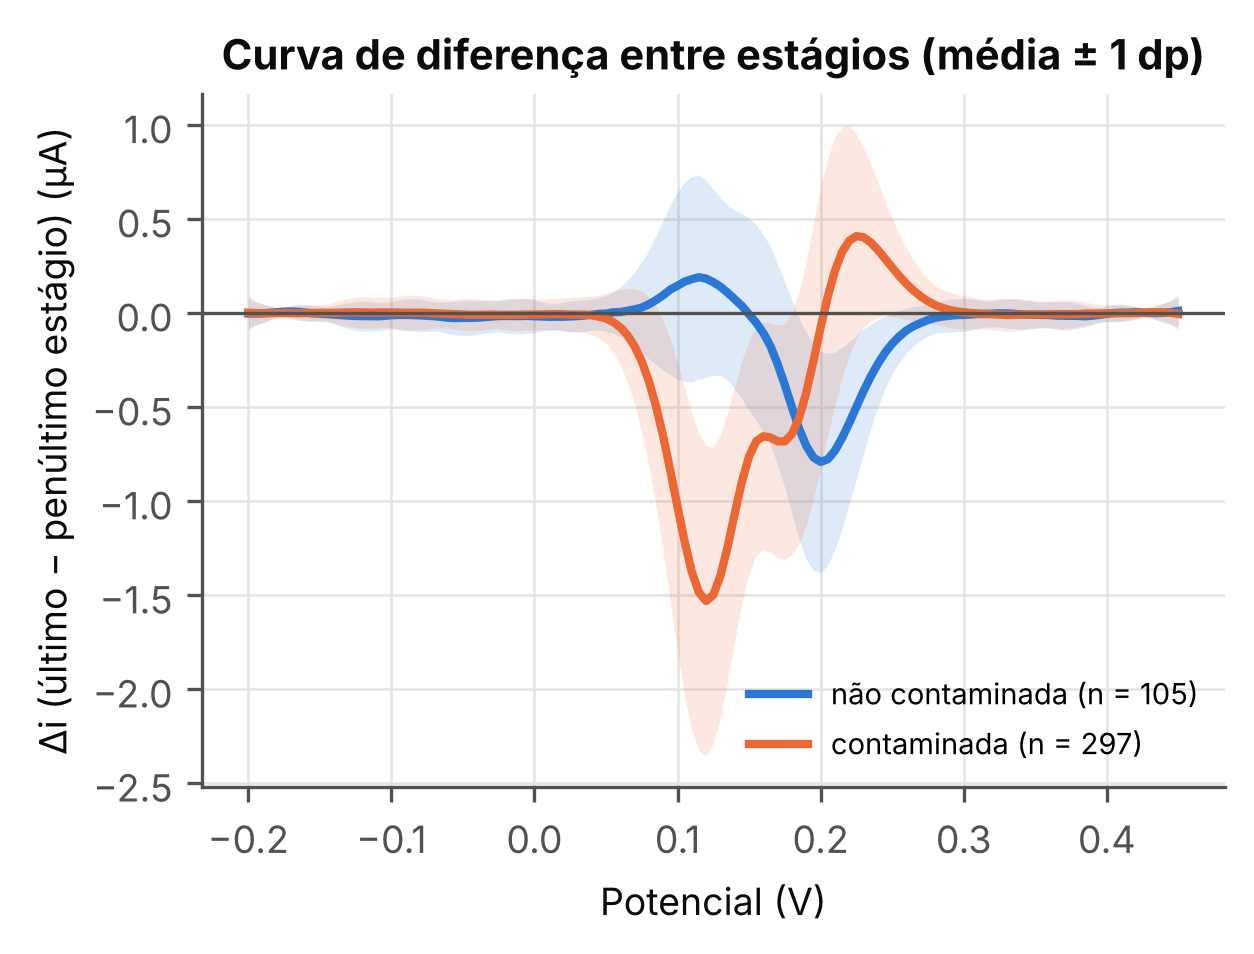
\includegraphics[width=0.62\textwidth]{curvas_diferenca.png}
\caption{Curva de diferença entre estágios (média $\pm$ 1 desvio-padrão) por classe, conjunto de treino.}
\label{fig:curvas}
\end{figure}

\subsection{Comparação de representações e modelos}
Foram avaliadas \NCombinacoes{} combinações (Figura~\ref{fig:comparacao},
Tabela~\ref{tab:classificacao}). A combinação escolhida pela validação cruzada foi
\MelhorModelo{} com a representação \MelhorVariante, com acurácia balanceada de
\ABcv{} $\pm$ \ABcvDP{} e AUC de \AUCcv. No conjunto de teste, ela obteve acurácia balanceada de
\ABteste, sensibilidade de \SENSteste, especificidade de \ESPECteste{} e AUC de \AUCteste{}
(limiar de \Limiar).

\begin{figure}[H]
\centering
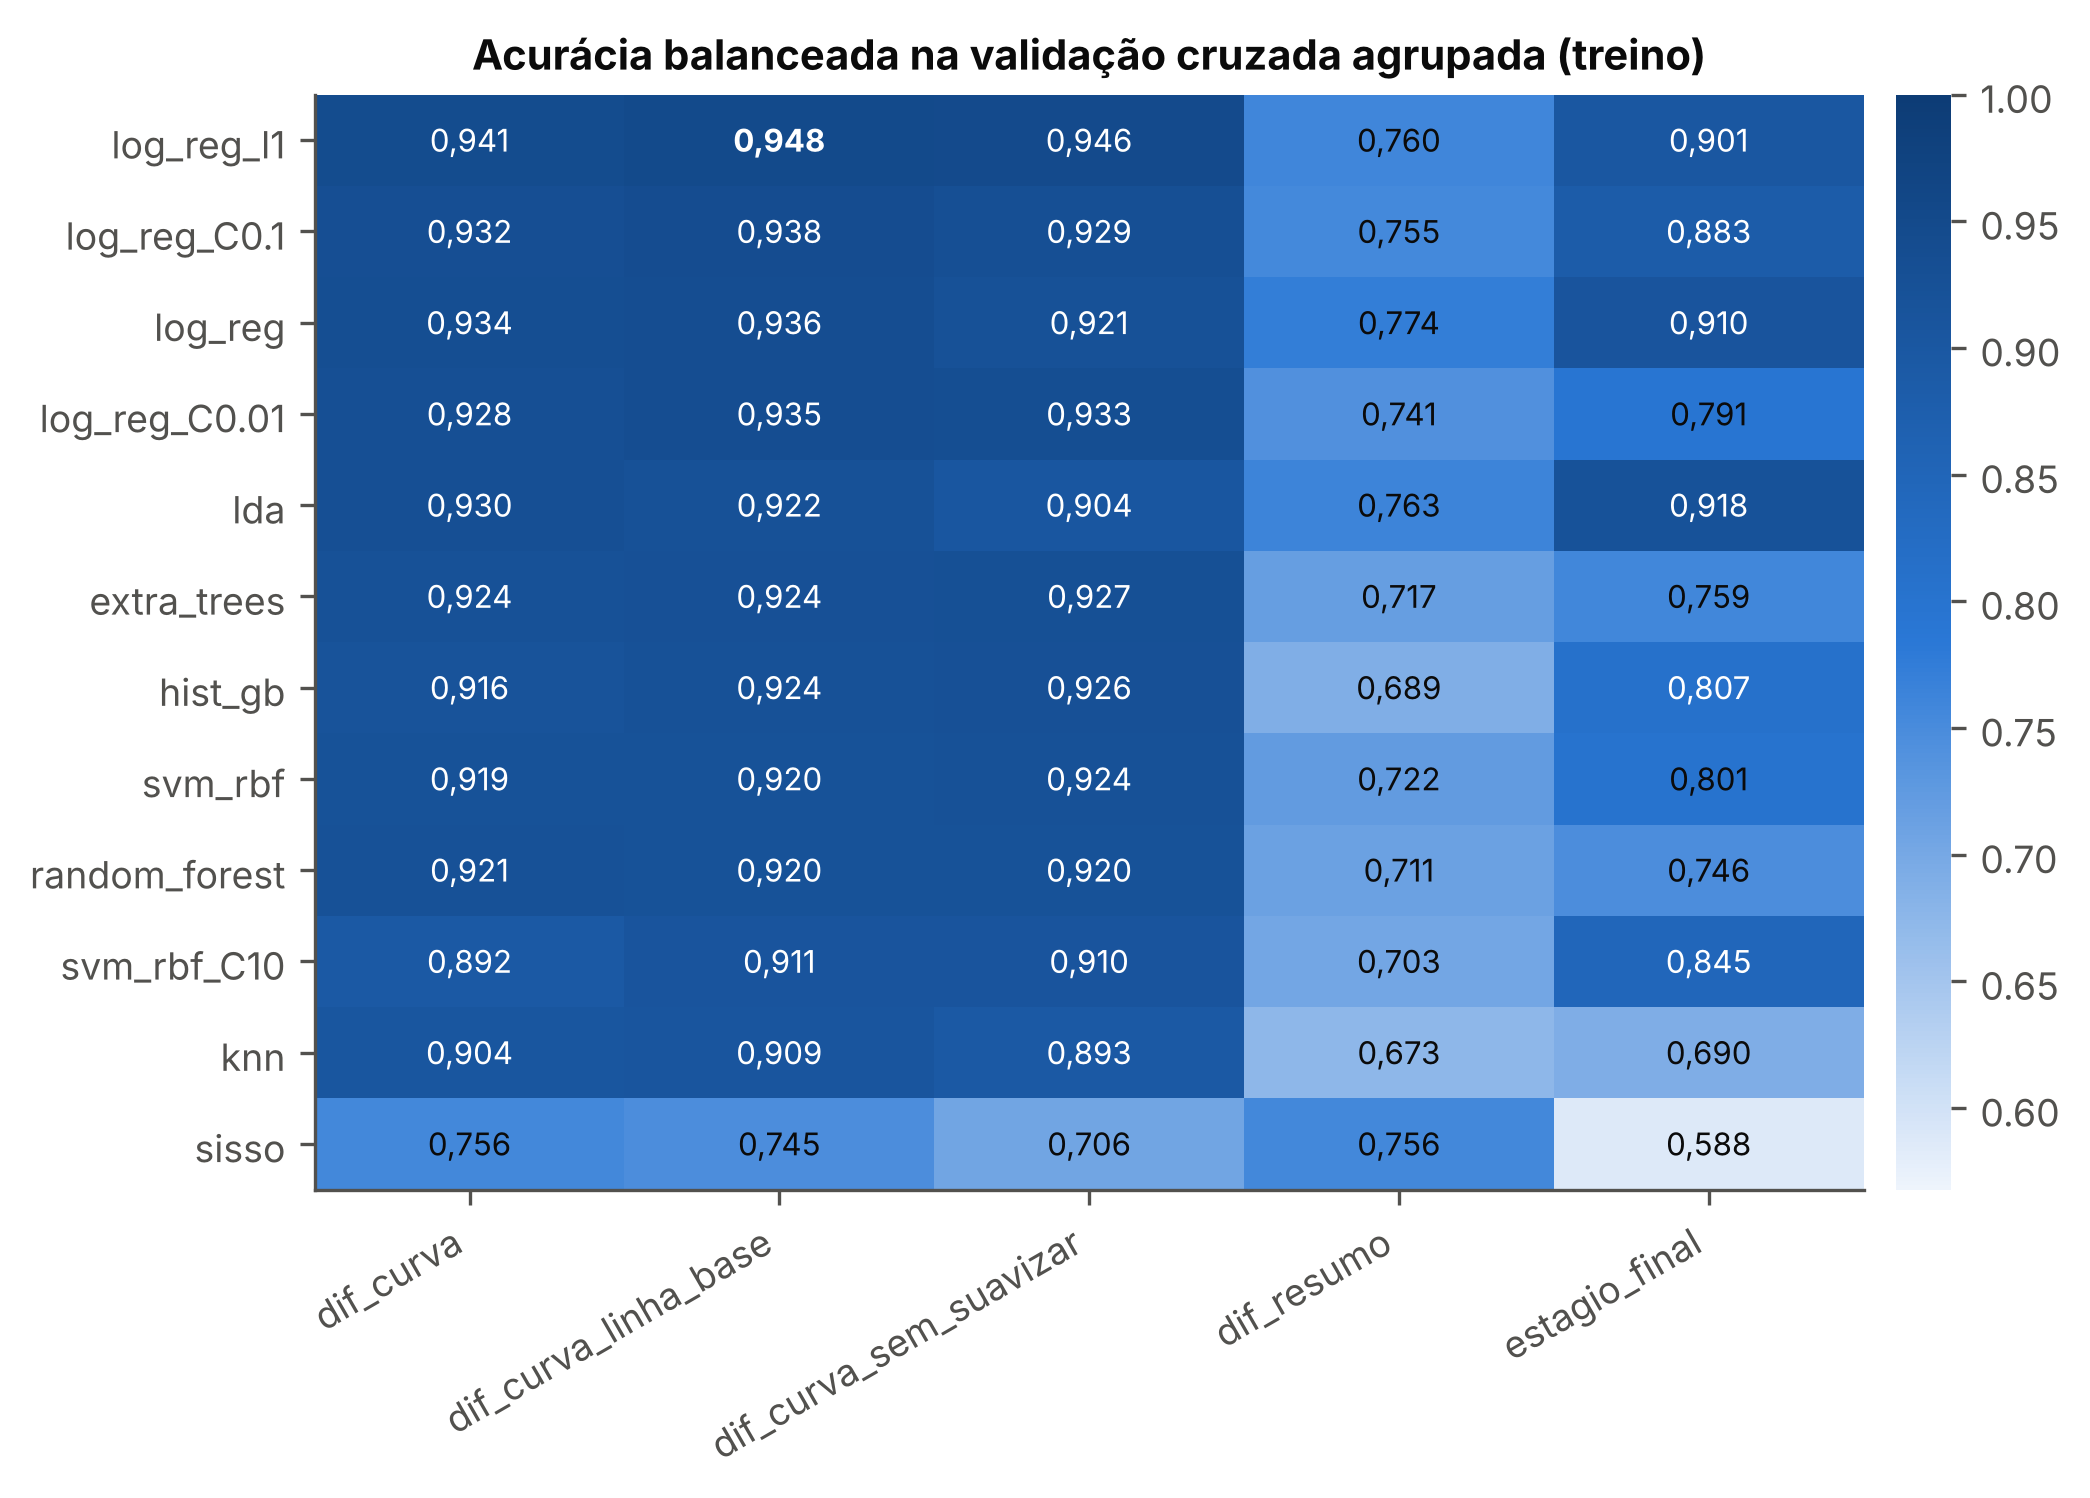
\includegraphics[width=0.9\textwidth]{comparacao_modelos.png}
\caption{Acurácia balanceada média na validação cruzada agrupada (treino) para cada representação e modelo.}
\label{fig:comparacao}
\end{figure}

\begin{table}[H]
\centering\footnotesize
\caption{Dez melhores combinações pela validação cruzada no treino e o desempenho de cada uma no
teste. AB: acurácia balanceada (média $\pm$ desvio-padrão entre dobras).}
\label{tab:classificacao}
\IfFileExists{gerado/tabelas/tabela_classificacao.tex}{\begin{tabular}{rllccccccc}
\toprule
 & & & CV (treino) & \multicolumn{2}{c}{Validação} & \multicolumn{4}{c}{Teste} \\
\cmidrule(lr){4-4}\cmidrule(lr){5-6}\cmidrule(lr){7-10}
\# & Variante & Modelo & AB & AB & AUC & AB & Sens. & Espec. & AUC \\
\midrule
1 & dif\_curva\_sem\_suavizar & log\_reg\_l1 & 0,941 $\pm$ 0,014 & 0,962 & 0,973 & 0,916 & 0,860 & 0,971 & 0,959 \\
2 & dif\_curva\_sem\_suavizar & log\_reg & 0,957 $\pm$ 0,019 & 0,957 & 0,971 & 0,889 & 0,892 & 0,886 & 0,941 \\
3 & dif\_curva\_sem\_suavizar & log\_reg\_C0.1 & 0,941 $\pm$ 0,017 & 0,952 & 0,973 & 0,921 & 0,871 & 0,971 & 0,951 \\
4 & dif\_curva\_linha\_base & log\_reg\_C0.01 & 0,938 $\pm$ 0,025 & 0,952 & 0,970 & 0,937 & 0,903 & 0,971 & 0,954 \\
5 & dif\_curva & lda & 0,955 $\pm$ 0,037 & 0,941 & 0,976 & 0,935 & 0,871 & 1,000 & 0,971 \\
6 & dif\_curva & log\_reg\_C0.1 & 0,941 $\pm$ 0,030 & 0,931 & 0,973 & 0,918 & 0,892 & 0,943 & 0,959 \\
7 & dif\_curva\_linha\_base & lda & 0,952 $\pm$ 0,037 & 0,930 & 0,974 & 0,930 & 0,860 & 1,000 & 0,970 \\
8 & dif\_curva & log\_reg\_l1 & 0,938 $\pm$ 0,019 & 0,926 & 0,973 & 0,903 & 0,892 & 0,914 & 0,960 \\
9 & dif\_curva & log\_reg & 0,949 $\pm$ 0,041 & 0,926 & 0,973 & 0,875 & 0,892 & 0,857 & 0,955 \\
10 & dif\_curva\_linha\_base & log\_reg\_l1 & 0,949 $\pm$ 0,033 & 0,925 & 0,974 & 0,918 & 0,892 & 0,943 & 0,958 \\
\bottomrule
\end{tabular}
}{\preencher{rodar fiep experimento --artigo}}
\end{table}

\begin{figure}[H]
\centering
\begin{subfigure}{0.48\textwidth}\centering
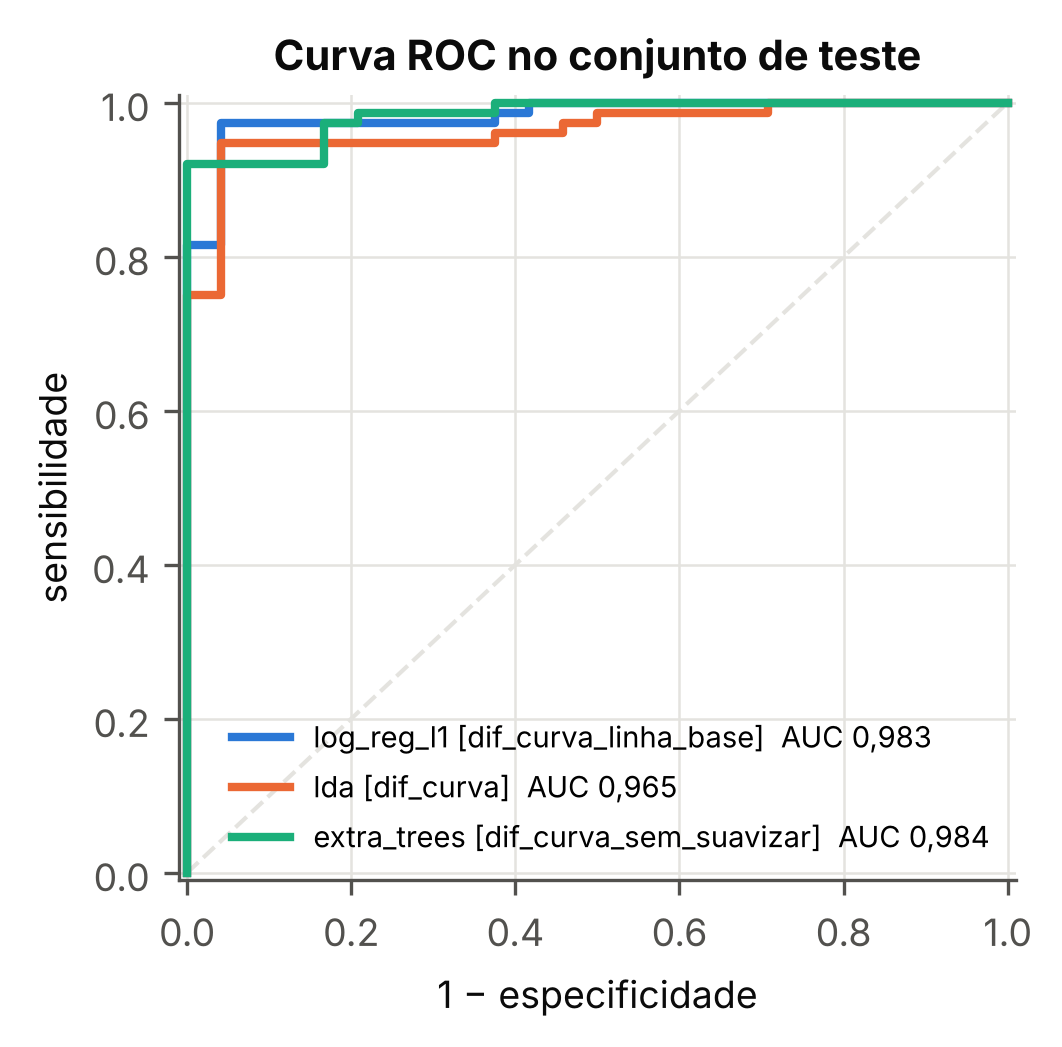
\includegraphics[width=\textwidth]{roc_teste.png}\caption{Curvas ROC no teste.}\end{subfigure}
\hfill
\begin{subfigure}{0.42\textwidth}\centering
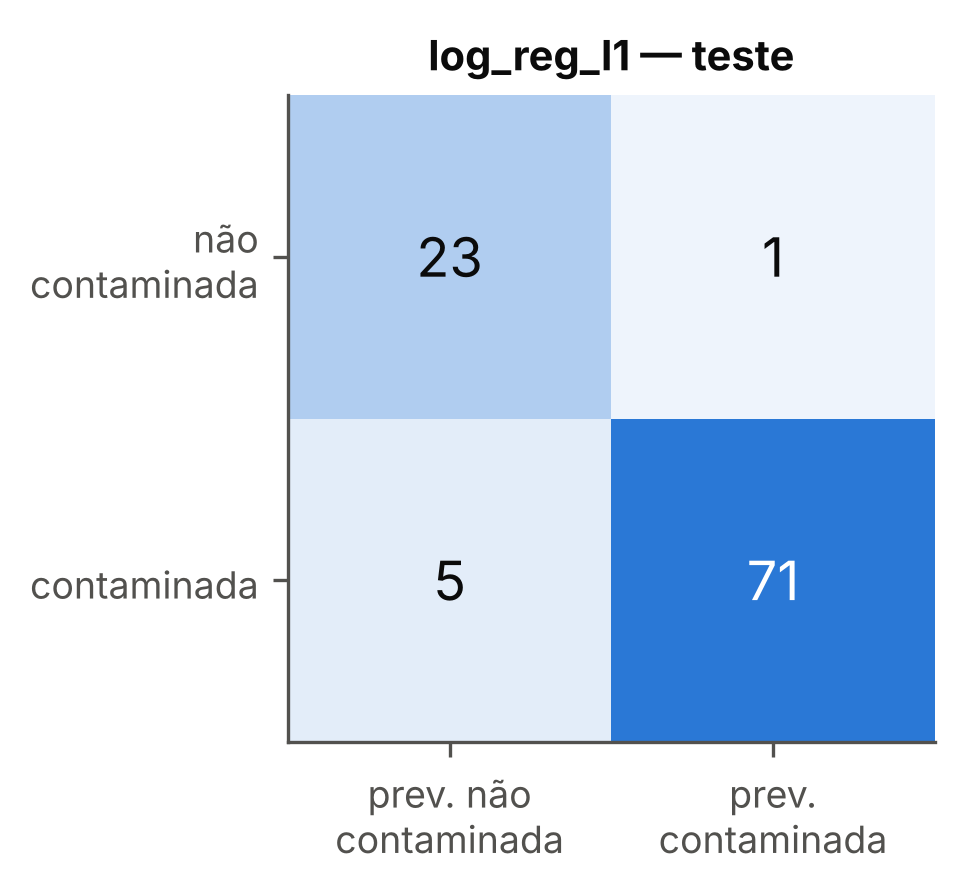
\includegraphics[width=\textwidth]{matriz_confusao_teste.png}\caption{Matriz de confusão do modelo escolhido.}\end{subfigure}
\caption{Desempenho no conjunto de teste.}
\label{fig:teste}
\end{figure}

\subsection{Interpretação}
A importância por permutação (Figura~\ref{fig:importancia}) indica as regiões de potencial que mais
pesam na decisão. O SISSO simplificado encontrou o descritor
\begin{center}\small\FormulaSISSO\end{center}
cuja forma explícita permite discutir o mecanismo com a equipe experimental.

\begin{figure}[H]
\centering
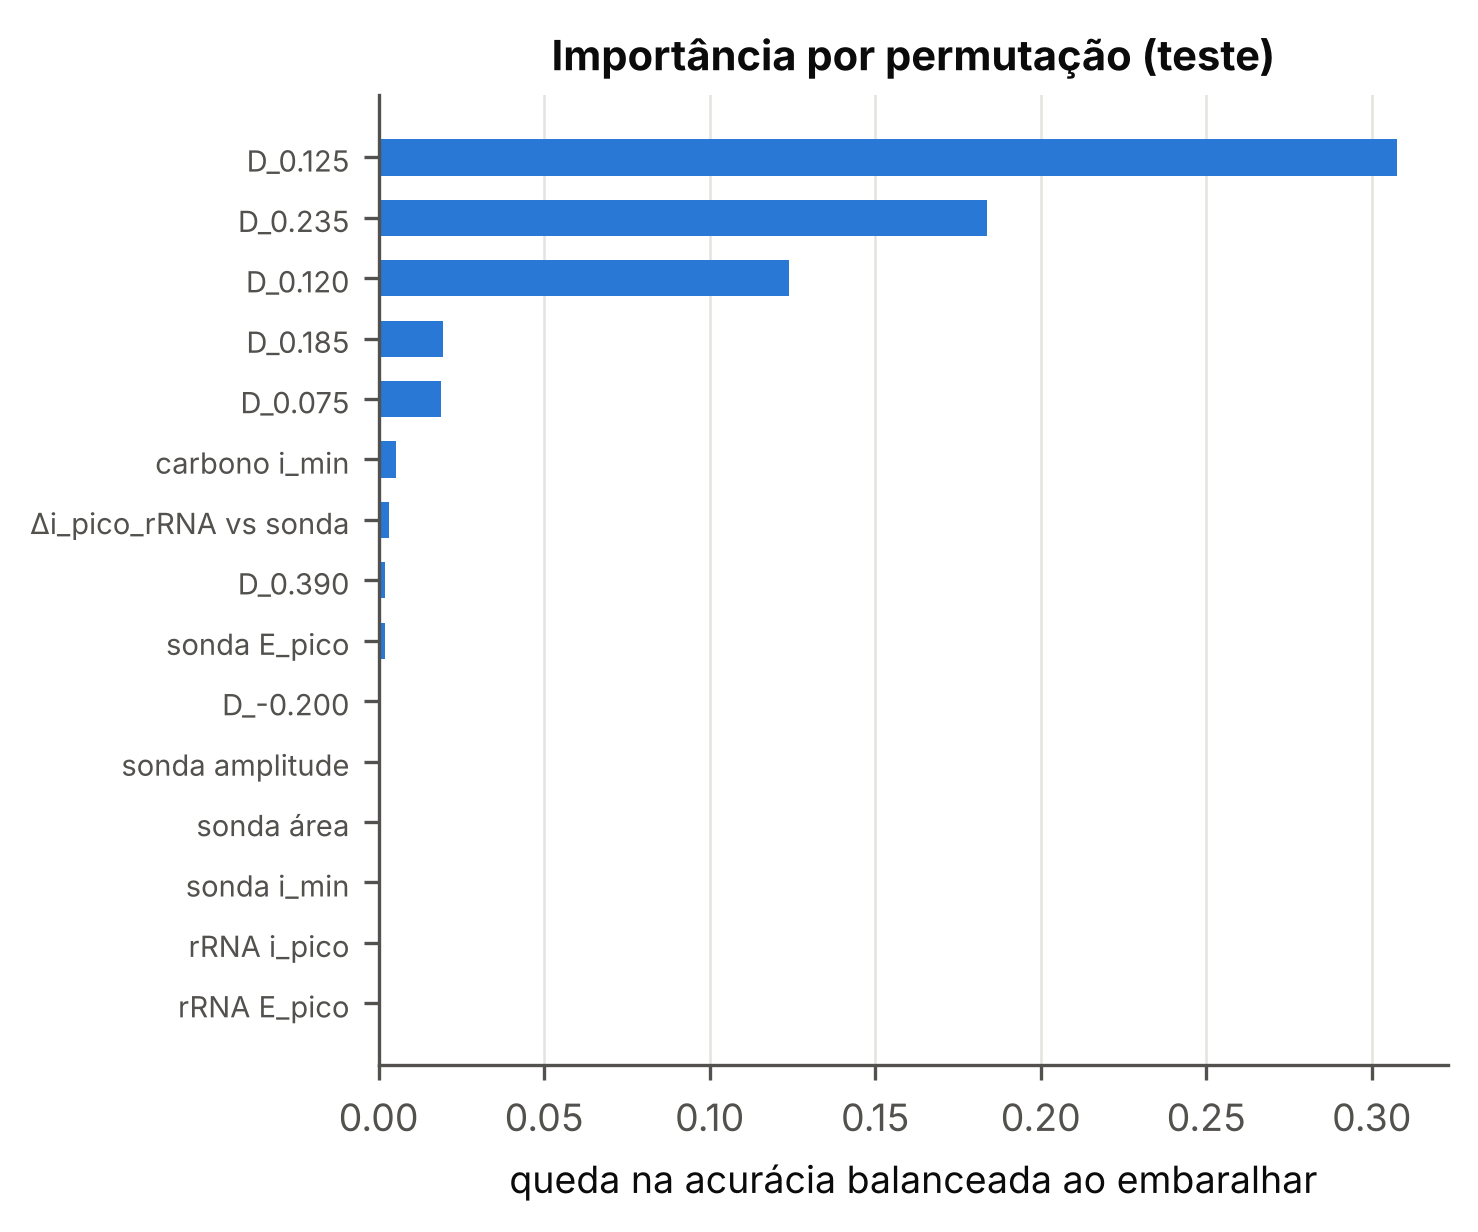
\includegraphics[width=0.6\textwidth]{importancia.png}
\caption{Importância por permutação das características no conjunto de teste (queda da acurácia balanceada).}
\label{fig:importancia}
\end{figure}

\subsection{Estimativa da carga bacteriana}
Nas amostras contaminadas, o melhor regressor (\RegModelo) teve RMSE de \RegRMSEcv{}
log$_{10}$\,UFC/mL na validação cruzada e de \RegRMSEteste{} no teste ($R^2 = \RegRdoisTeste$)
(Tabela~\ref{tab:regressao}, Figura~\ref{fig:regressao}).

\begin{table}[H]
\centering\small
\caption{Regressão da carga bacteriana (log$_{10}$\,UFC/mL) nas amostras contaminadas.}
\label{tab:regressao}
\IfFileExists{gerado/tabelas/tabela_regressao.tex}{\begin{tabular}{llcccc}
\toprule
 & & \multicolumn{2}{c}{Validação cruzada} & \multicolumn{2}{c}{Teste} \\
\cmidrule(lr){3-4}\cmidrule(lr){5-6}
Variante & Modelo & RMSE & $R^2$ & RMSE & $R^2$ \\
\midrule
dif\_curva\_linha\_base & ridge & 0,79 & 0,72 & 0,81 & 0,66 \\
dif\_curva\_linha\_base & pls & 0,82 & 0,70 & 0,86 & 0,61 \\
dif\_curva\_linha\_base & svr & 0,92 & 0,62 & 0,92 & 0,55 \\
dif\_curva\_linha\_base & hist\_gb & 0,93 & 0,62 & 1,05 & 0,42 \\
dif\_curva\_linha\_base & extra\_trees & 0,98 & 0,58 & 1,05 & 0,42 \\
dif\_curva\_linha\_base & random\_forest & 1,01 & 0,55 & 1,10 & 0,36 \\
dif\_resumo & ridge & 1,06 & 0,50 & 1,02 & 0,45 \\
dif\_resumo & pls & 1,06 & 0,50 & 1,05 & 0,42 \\
dif\_resumo & extra\_trees & 1,13 & 0,44 & 1,20 & 0,24 \\
dif\_resumo & random\_forest & 1,15 & 0,41 & 1,30 & 0,11 \\
dif\_resumo & hist\_gb & 1,16 & 0,41 & 1,20 & 0,24 \\
dif\_resumo & svr & 1,27 & 0,29 & 1,39 & -0,02 \\
\bottomrule
\end{tabular}
}{\preencher{rodar fiep experimento --artigo}}
\end{table}

\begin{figure}[H]
\centering
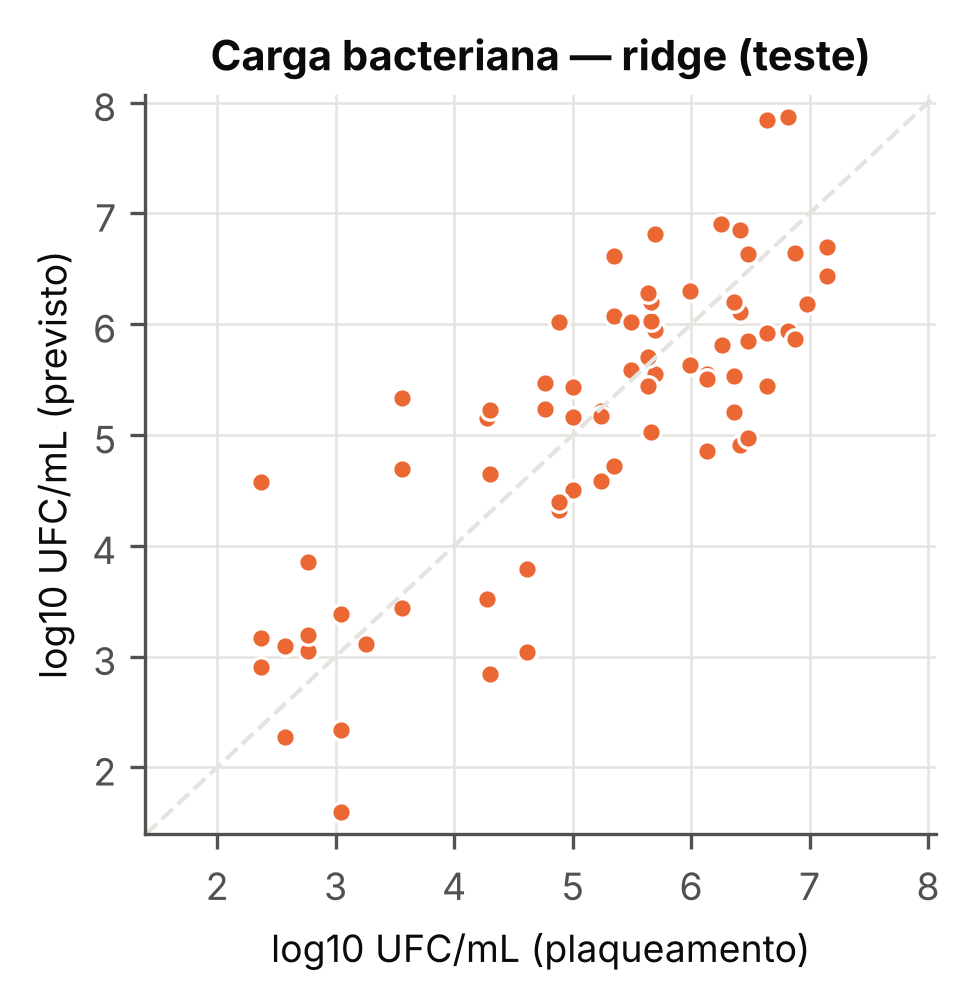
\includegraphics[width=0.45\textwidth]{regressao_teste.png}
\caption{Carga prevista versus plaqueamento no conjunto de teste.}
\label{fig:regressao}
\end{figure}
